
% This .tex file (and associated .cls) produces:
%       1) The Permission Statement
%       2) The Conference (location) Info information
%       3) The Copyright Line TSConIT
%       4) NO page numbers
%       5) NO headers and/or footers
%
% Using 'sig-alternate.cls' you have control, however, from within
% the source .tex file, over both the CopyrightYear
% (defaulted to 200X) and the ACM Copyright Data
% (defaulted to X-XXXXX-XX-X/XX/XX).
% e.g.
% \CopyrightYear{2007} will cause 2007 to appear in the copyright line.
% \crdata{0-12345-67-8/90/12} will cause 0-12345-67-8/90/12 to appear in the copyright line.
%
% ---------------------------------------------------------------------------------------------------------------
% This .tex source is an example which *does* use
% the .bib file (from which the .bbl file % is produced).
% REMEMBER HOWEVER: After having produced the .bbl file,
% and prior to final submission, you *NEED* to 'insert'
% your .bbl file into your source .tex file so as to provide
% ONE 'self-contained' source file.
%

% refers to the cls file being used
\documentclass{sig-alternate-br}
\usepackage{float}
\usepackage{caption}
\usepackage{subcaption}
\usepackage{hyperref}

\restylefloat{figure}
\restylefloat{table}
\begin{document}

%
% --- Author Metadata here --- DO NOT REMOVE OR CHANGE 
%\conferenceinfo{13$^{th}$ Twente Student Conference on IT}{June 23$^{st}$, 2010, Enschede, The Netherlands.}
\CopyrightYear{2015} % Allows default copyright year (200X) to be over-ridden - IF NEED BE.
%\crdata{0-12345-67-8/90/01}  % Allows default copyright data (0-89791-88-6/97/05) to be over-ridden - IF NEED BE.
% --- End of Author Metadata ---

\title{micro data server using raspberry pi}
% In Bachelor Referaat at University of Twente the use of a subtitle is discouraged.
 \subtitle{Research Proposal}




\numberofauthors{1} 
\author{ 
% You can go ahead and credit any number of authors here,
% e.g. one 'row of three' or two rows (consisting of one row of three
% and a second row of one, two or three).
%
% The command \alignauthor (no curly braces needed) should
% precede each author name, affiliation/snail-mail address and
% e-mail address. Additionally, tag each line of
% affiliation/address with \affaddr, and tag the
% e-mail address with \email.
%
% 1st. author
\alignauthor P.j.e. Velthuis\\
       \affaddr{University of Twente}\\
       \affaddr{P.O. Box 217, 7500AE Enschede}\\
       \affaddr{The Netherlands}\\
       \email{p.j.e.velthuis@student.utwente.nl}
% 2nd. author
\alignauthor 2nd Author\\
       \affaddr{2nd author's affiliation}\\
       \affaddr{1st line of address}\\
       \affaddr{2nd line of address}\\
       \email{2nd author's email address}
% 3rd. author
\alignauthor 3rd Author\\
       \affaddr{3rd author's affiliation}\\
       \affaddr{1st line of address}\\
       \affaddr{2nd line of address}\\
       \email{3rd author's email address}
}

%\additionalauthors{Additional authors: John Smith (The
%Th{\o}rv{\"a}ld Group, email: {\texttt{jsmith@affiliation.org}})
%and Julius P.~Kumquat (The Kumquat Consortium, email:
%{\texttt{jpkumquat@consortium.net}}).}
%\date{30 July 1999}


\maketitle
\begin{abstract}
This document describes a draft research proposal in the
area of cloud computing services. The main research question
is: What is the performance of raspberry pi load balancing service using video streaming? To answer this question a micro raspberry pi video streaming service will be build. 
\end{abstract}

\keywords{Cloud computing, Raspberry Pi, ARM performance, micro data server, video streaming, load balancing}

\section{Motivation}
Today there are many cloud services. This amount of cloud computing services is increasing fast \cite{armbrust:2009}.  Despite the attention
from the research community, research and development of
Cloud Computing services is still in it's childhood\cite{tso:2013}. 
In this research the Raspberry Pi cloud services will be investigated. A reason for this is that the density of servers has increased a lot in the past\cite{density}. There are new technologies such as for example the ARM processor. Many companies want to explore the possibilities of for example the Raspberry Pi and his ARM Processor. Some data centers even offer some cloud computing using the Raspberry Pi. A reason for this is the co-location and the low power usage of a Raspberry Pi\cite{hosting,Pcextreme}.  A Raspberry Pi has a power usage between the 3-5 Watt. A normal server has a power usage between the 75 and 150 watt \cite{Powerusage}. This could mean that it is better to use a Raspberry Pi for specific small tasks that do not demand a whole server. During this research I want to further investigate the performance of the Raspberry pi as a server.  A Raspberry Pi can be the small data center for the future \cite{tso:2013}. The Raspberry is a rather cheap device for 35 euros. This makes it cheaper to do research in compared to a normal server. This is also the mean reason why the Raspberry pi was ones created. The current versions of the Raspberry Pi cannot perform the task of a large scale x86 server \cite{tso:2013}. Building a cloud like this can be a cost effective scale model\cite{tso:2013}. It's a ideal testbed for testing distributed software. During this research we will investigate the performance of a raspberry pi as a video streamer to other computers. The reason I want to investigate it with video streaming is because this demands a lot of bandwidth from the network and could be one of the first things that should be improved. 

\section{Specific problem}

Today a lot of people watch their movies online using video streaming. 
The Netherlands have for example one million subscribers for Netflix \cite{volkskrant}. Netflix is a video streaming service that makes HD movies watching possible. For this Netflix makes use of a content distribution network (CDN). On the internet
this is also known as a on demand service \cite{Adhikari:2012}. Netflix makes use of
MPEG-DASH a protocol that makes streaming over http possible \cite{martin:2013}. The problem is that Netflix is responsible for  29.7\% of the peak downstream traffic in US  \cite{Adhikari:2012}. In the Netherlands more and more users are making use of video streaming as Youtube and Netflix.  In this research we want to investigate if it is possible to make small micro data centers with raspberry pi's. This research will try to find out how this cloud works. There will be taken a look in for example the load balancing of video streaming. In this way it can be possible to see improvements that can be made in the load balancing so that the servers can be used more efficient. This is also build to learn more from load balancing and a computer cluster. This can be really useful, because nowadays it's still done on relatively expensive servers. 


\section{Research questions}
The main research question
is: What is the performance of a raspberry pi load balancing service using video streaming?

In order to come to a good answer we need to  research several things

build our own Raspberry Pi setup. There needs to be decided with which benchmark the performance will be measured. After we have measured the performance we can see   


\subsection{What is small scale cloud computing?}
In this research I want to do some small scale cloud computing. The main motivation behind is is that it is ways to expensive to simulate large scale cloud computing. Another reason is the Co-location that can be used with small scale cloud computing. Because of this it could be better in executing small tasks. Small scale cloud computing is cloud computing with smaller computation amounts than normal. More motivation is that it does not use a lot of space and power. 
Resources I could use for small scale cloud computing:
\cite{Pcextreme,armbrust:2009,richardson:2012,abrahamsson:2013,southampton}
 


\subsection{What is cloud video streaming}
There are a lot of cloud services nowadays. These include a webserver, a DNS server, a chat server, a mail server, a vpn server or a monitoring server or even a video streaming service. 
Today a lot of people watch their movies online using video streaming. The netherlands have for example one million subscribers for Netflix \cite{volkskrant}. Netflix is a video streaming service that makes HD movies watching possible. For this Netflix makes use of a content distribution network (CDN). On the internet this is also known as a on demand service. They make use of amazon its AWS with a AWS cloud, Amazon simpleDB , S3 and cassandra for file storage \cite{Adhikari:2012}. Netflix makes use of MPEG-DASH a protocol that makes streaming over http possible. In this research I want to investigate more in the video streaming as a cloud service. 
To investigate this I want to make a experimentation cloud with Raspberry Pi's to see if it will work as a cloud. 
Resources I could use for cloud video streaming:
\cite{g-streamer,raspberry-video,video-1080p, plissonneau:2012}
 
\subsection{What kind of different load balancing techniques are there?}
In distributed servers it is very important that good load balancing takes place. For this reason I want to further investigate in what kind of load balancing techniques there are. 
Resources I could use for load balancing:
\cite{nginx-load-balancing,nginx-load-balancing-2,computer-networking,wolf:1997,load-balancing}

 
\subsection{Is it reachable to build small personal Raspberry Pi clouds for services}
With this subquestion I want to find out if it is possible to let users have small Raspberry Pi servers I also want to know what the performance of this small Raspberry Pi cloud is. 
Resources:
\cite{Pcextreme,nginx-load-balancing,nginx-load-balancing-2}

\subsection{Is it possible to improve load balancing using small scale Raspberry Pi's}
For this research I want to investigate if it is possible to do more research in the 
load balancing techniques that can be used in a raspberry pi. A example of this would be the round robin protocol.
Resources:
\cite{nginx-load-balancing,nginx-load-balancing-2}

\section{Research Methods}
This research will investigate a cloud computer consisting of Raspberry Pi's. The research method for this would be the Design Science research method. this is a method to solve field problems. This research will make use of the design Science method proposed by Hevner\cite{hevner:2007}.

\section{Research approach}
For the experiment we need a Raspberry Pi with a static Ip address and we need a sd card for the OS. For the experiment we need a Raspberry Pi B that can make use of the Ethernet. This is because a Raspberry Pi can be used as a webserver and this is needed to have this in order to make video streaming possible. This webserver will make video streaming possible. It will have a VPN to make it possible to put video's on the Raspberry pi \cite{VPN:2014}. 
So I will first make this video streaming webserver. 
After this we will make a cluster with one Raspberry Pi as a load balancer and the other two as a video stream pi. If I have made such I cluster I can start doing some tests on it. For example some test in streaming in different quality with load balancing. The setup of the raspberry Pi can be seen in the figure below ~\ref{fig:setup}.

\begin{figure}[H]
\centering 
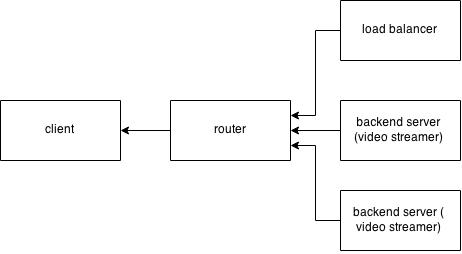
\includegraphics[width=0.4\textwidth]{raspberry pi setup.jpg}
\caption{Insert caption to place below figure.}
\label{fig:setup} %always place your label after your caption!
\end{figure}
For the load balancing we will make use of Nginx for this we will use the following sources:
\cite{nginx-load-balancing, nginx-load-balancing-2}


\section{Planning}

\begin{table}[H]
	\centering \caption{Planning}
\begin{tabular}{|c|c|c|} \hline
		\textbf{Week} & \textbf{Date} & \textbf{Activity} \\ \hline 
		6-9& 6 Feb. -27 Feb& Collect literature and software\\ \hline 
		10& 2 March - 9 March& Deadline peer review and proposal \\ \hline
		12& 16 March -22 March & \textbf{Deadline proposal} \\ \hline
		13 & 23 March -30 March &  \textbf{Accept Reject proposal} \\ \hline
		10-14& 2 March 12 April& Start building test environment \\ \hline
		14& 6 April - 12 April& Answer subquestion 1  \\ \hline
		15& 13 April - 20 April& Answer subquestion 2\\ \hline
		16& 21 April - 28 April& Answer subquestion 3\\ \hline
		14-16 & 6 April - 28 April & working on test environment \\ \hline
		17& 1 May - 7 May & Answer subquestion 4 \\ \hline
		18& 4 May-10 May& conclusion and check coherency \\ \hline
		19& 11 May-18 May& Finalize paper \\ \hline
		22& 1 June-7 June&  \textbf{Deadline paper} \\ \hline
		26 &22 June - 26 June & \textbf{Conference} \\ \hline
		\end{tabular}

		\label{tab:planning}
\end{table}
Here above is the table~\ref{tab:planning}. The main research question is split up into several sub questions. These subquestions have each one week for answering. After that there is time to write the conclusion and answer the main question. Then there is still some time left to finalize the paper. 

\section{State of the Art}
Today there are many cloud services. This amount of cloud computing services is increasing fast \cite{armbrust:2009}.  Despite the attention
from the research community, research and development of
Cloud Computing services is still in it's childhood\cite{tso:2013}. Today there is a lot of people that use video streaming and this will become even more. People want to have everything has to be accessible through the network around the clock \cite{youseff:2008}. One thing that people want on demand are there film series. Currently Netflix has 30\% of the downstream in the United States. This downstream is huge and that means that there is optimization in this branch possible. To make the video on demand service of Netflix possible they use servers from Amazon. 

In this paper there will be research done on making a load balancing service for the Raspberry Pi.  This service will consist of several raspberry Pi's. These Raspberry Pi's make together a small cloud computer.  The Raspberry Pi is made for research and education purposes \cite{raspberry-pi}. The Raspberry Pi is a cheap device costing around 35 euro. It has a power consumption of only three watt and has quite good processor. For this reason it might be very useful for small scale cloud computing. The raspberry Pi is a small device and is excellent for a lot of small devices in a relatively small place. The Raspberry Pi doesn't use cooling and it can be used for very rapid elasticity and on-demand self-service. Because of it's cooling features and low power consumption it might be a good alternative for the nowadays high power consuming data centers. The raspberry pi is really small so it is a lot easier to place extra pi in a data center compared to a normal server. The Raspberry Pi has one drawback and that is that the processing power is relatively low. By using load balancing there will be taken a look at what load balancing techniques are successful for the Raspberry pi. 

In this research we will make a small raspberry cloud to do research on video streaming using HTTP. This will be done using the design Science method proposed by Hevner\cite{hevner:2007}. After we have done this for the Raspberry Pi there will be looked at streaming using Amazon. In this way we can see how the results are compared to streaming via Amazon. This research will try to find out if the raspberry has enough processing power to stream to multiple web clients. The cloud performance can now be better researched, because everything is at one location and the information about what processes are running on the pi are well defined. In this way we can take a better look at algorithms used in video streaming. This is mostly because there is not a lot of overhead. 


\bibliographystyle{abbrv}
\bibliography{sigproc}  % sigproc.bib is the name of the Bibliography in this case
% You must have a proper ".bib" file
%  and remember to run:
% latex bibtex latex latex
% to resolve all references
%
% ACM needs 'a single self-contained file'!
%
\vspace{50 mm}
\newpage
%APPENDICES are optional


\end{document}
